%
%  D0018E report 1
%
%  Created by Anders Lindmark on 2012-10-31.
%  Copyright (c) 2011 Anders Lindmark. All rights reserved.
%
%\documentclass[]{article}
\documentclass[12pt, a4paper,titlepage]{article}

% Use utf-8 encoding for foreign characters
\usepackage[utf8]{inputenc}
\usepackage[english]{babel}

% Setup for fullpage use
\usepackage{fullpage}

\usepackage{float}
\usepackage[T1]{fontenc}
% Uncomment some of the following if you use the features
%
% Running Headers and footers
%\usepackage{fancyhdr}

% Multipart figures
%\usepackage{subfigure}

% More symbols
\usepackage{amsmath}
%\usepackage{amssymb}
%\usepackage{latexsym}

% Surround parts of graphics with box
\usepackage{boxedminipage}

% Package for including code in the document
\usepackage{listings}

% If you want to generate a toc for each chapter (use with book)
\usepackage{minitoc}

% This is now the recommended way for checking for PDFLaTeX:
\usepackage{ifpdf}

%\newif\ifpdf
%\ifx\pdfoutput\undefined
%\pdffalse % we are not running PDFLaTeX
%\else
%\pdfoutput=1 % we are running PDFLaTeX
%\pdftrue
%\fi

\ifpdf
\usepackage[pdftex]{graphicx}
\else
\usepackage{graphicx}
\fi

\usepackage{tikz}
\usetikzlibrary{positioning,arrows,fit,shapes,calendar,chains}
\usetikzlibrary{shadows}



\usepackage{tikz-er2} % For Entity-Relationship diagrams

\usepackage{pgfplots}
\usepackage{pgfplotstable}

\usepackage{hyperref}

\usepackage{enumerate}

\usepackage{todonotes}

%\usepackage{eso-pic}

\usepackage{color}
\definecolor{error}{RGB}{193,27,23} % #C11B17, Firebrick3
\definecolor{warning}{RGB}{229,103,23} % #E56717, Dark Orange2
%\definecolor{codebg}{RGB}{245,245,245}
\definecolor{codebg}{RGB}{247,247,247}
\definecolor{dkgreen}{rgb}{0,0.6,0}
\definecolor{poop}{rgb}{0.82,0.71,0.15}

\usepackage{parskip}
\setlength{\parskip}{0.4cm}
\setlength{\parindent}{0.6cm}

%\title{\huge\sffamily D7001D  Home examination}
%\author{Anders Lindmark, \emph{830604-8995}}
%\date{\today}

% http://tex.stackexchange.com/questions/16501/problem-with-special-characters-in-listings
%\lstset{literate=%
%{å}{{\aa}}1
%ä}{{\"a}}1
%{ö}{{\"o}}1
%{Å}{{\AA}}1
%{Ä}{{\"A}}1
%{Ö}{{\"O}}1
%}
\lstdefinelanguage{pseudo}{morekeywords={for,if,else,do,then,to,return,while,break}}
\lstset{
%backgroundcolor=\color{lightgray},
backgroundcolor=\color{codebg},
%title=\lstname,
frame=lines,
%inputencoding=utf8,
inputencoding=ansinew,
extendedchars=\true,
%basicstyle=\small,
basicstyle=\small,
commentstyle=\color{red},
numberstyle=\footnotesize\color{gray},
stringstyle=\color{poop},
breaklines=true,
%keywordstyle=\color{black}\bfseries,
language=Python,
numbers=left,
}


\begin{document}
\ifpdf
\DeclareGraphicsExtensions{.pdf, .jpg, .tif}
\else
\DeclareGraphicsExtensions{.eps, .jpg}
\fi

\begin{titlepage}
\ 
\begin{center}
\vfill
{\huge\sffamily D0018E Report (3+4)}
\rule{\linewidth}{0.3mm}\\
Anders Lindmark \\
\vfill
\ 
\vfill
{\textbf{\today}}
\end{center}
\end{titlepage}

\tableofcontents
\newpage

\section{Establish a minimalistic website}
\subsection{Development environment}
The framework I have chosen to use is
Django\footnote{\url{https://www.djangoproject.com/}}. 
It is a framework that I have previous experience with and which I think is
very powerful aswell as easy to get started with.
It has a very good object-relational mapper (ORM) for working with databases as well
as support for running raw SQL-queries which are then mapped into objects
automatically using the ORM.

There are probably many good IDE's for developing in python/Django, NetBeans
being the one I usually use, but I will work with the editor \emph{vim}. It is the 
editor I'm most comfortable with, and vim combined with
\emph{screen}\footnote{\url{http://www.gnu.org/software/screen/}} and an
ssh-client enables me to switch computers and continue working where I left
off without having to install an IDE and download/upload code.

I will use \emph{git}\footnote{\url{http://git-scm.com/}} to keep track of code
and documentation changes which also enables me to go back to a point in
time incase I forget to document something in one of these hand-ins.

\subsection{The database}
Since I am developing on my own server I will use the 
\emph{MySQL}-installation already present on it.
I have started modelling the tables that I think I need for this application, using
the Django modelling system. When using this system you define a set of 
objects that represent the different tables and their columns. You can easily
specify relationships between the tables aswell. 

\subsubsection{Django models}
\label{sec:djangomodels}
The models that I have come up with so far, and these might change in the
future when more work is done, are:

\begin{itemize}
\setlength\itemsep{-1pt}
\item Customer - A user on the site. Django has a user-system already and this
model extends that system with the extra information we need.
\begin{lstlisting}
class Customer(models.Model):
    """ 
    Contains extra information about a customer other than the fields that are available in django-auth.
    """
    # For now, store all address info in one field, i.e "Bob Bobster\n13Bob street\nBobtown"
    address = models.CharField(max_length=150) 
    phone_number = models.CharField(max_length=20)
    user = models.OneToOneField(User) # The user-field points into Django's own auth-system.
\end{lstlisting}

\item Category - Different categories of products
\begin{lstlisting}
class Category(models.Model):
    """ 
    Represents a group of specific assets, i.e if we are selling food then "Snacks" could be a category
    """
    name = models.CharField(max_length=50)
    description = models.CharField(max_length=150)
\end{lstlisting}

\item Asset - The different products themselves
\begin{lstlisting}
class Asset(models.Model):
    """ 
    Represents a product.
    """
    name = models.CharField(max_length=50)
    description = models.CharField(max_length=150)
    category = models.ForeignKey(Category) # Which category does this asset belong to
    stock = models.IntegerField() # How many of this asset are in stock
\end{lstlisting}

\item Basket - The current shopping basket for a specific customer
\begin{lstlisting}
class Basket(models.Model):
    """
    Shopping basket, contains a list of assets and which customer it belongs to.
    """
    assets = models.ManyToManyField(Asset)
    customer = models.ForeignKey(Customer)
\end{lstlisting}

\item Order - A placed order
\begin{lstlisting}
class Order(models.Model):
    """
    A placed order, contains information about which assets was ordered, which customer placed the order and
    when the order was placed/shipped.
    """
    assets = models.ManyToManyField(Asset)
    customer = models.ForeignKey(Customer)
    date_placed = models.DateTimeField(auto_now=True) # Date the order was placed
    date_filled = models.DateTimeField() # Date the order was filled 
\end{lstlisting}
\end{itemize}

\subsubsection{SQL models}
\label{sec:sqlmodels}
Django takes the models that you have created and outputs SQL-code.
Normally this is done behind the scenes but you can get the SQL-code used
to create the tables. The code for the current version of my models looks like
this:

\lstset{language=SQL}
\begin{lstlisting}
CREATE TABLE `shopping_customer` (
    `id` integer AUTO_INCREMENT NOT NULL PRIMARY KEY,
    `address` varchar(150) NOT NULL,
    `phone_number` varchar(20) NOT NULL,
    `user_id` integer NOT NULL UNIQUE
)
;
ALTER TABLE `shopping_customer` ADD CONSTRAINT `user_id_refs_id_40cf930a` FOREIGN KEY (`user_id`) REFERENCES `auth_user` (`id`);

CREATE TABLE `shopping_category` (
    `id` integer AUTO_INCREMENT NOT NULL PRIMARY KEY,
    `name` varchar(50) NOT NULL,
    `description` varchar(150) NOT NULL
)
;
CREATE TABLE `shopping_asset` (
    `id` integer AUTO_INCREMENT NOT NULL PRIMARY KEY,
    `name` varchar(50) NOT NULL,
    `description` varchar(150) NOT NULL,
    `category_id` integer NOT NULL,
    `stock` integer NOT NULL
)
;
ALTER TABLE `shopping_asset` ADD CONSTRAINT `category_id_refs_id_71ff6d8a` FOREIGN KEY (`category_id`) REFERENCES `shopping_category` (`id`);

CREATE TABLE `shopping_basket_assets` (
    `id` integer AUTO_INCREMENT NOT NULL PRIMARY KEY,
    `basket_id` integer NOT NULL,
    `asset_id` integer NOT NULL,
    UNIQUE (`basket_id`, `asset_id`)
);
ALTER TABLE `shopping_basket_assets` ADD CONSTRAINT `asset_id_refs_id_4c78df9` FOREIGN KEY (`asset_id`) REFERENCES `shopping_asset` (`id`);

CREATE TABLE `shopping_basket` (
    `id` integer AUTO_INCREMENT NOT NULL PRIMARY KEY,
    `customer_id` integer NOT NULL
);
ALTER TABLE `shopping_basket` ADD CONSTRAINT `customer_id_refs_id_20577cdd` FOREIGN KEY (`customer_id`) REFERENCES `shopping_customer` (`id`);
ALTER TABLE `shopping_basket_assets` ADD CONSTRAINT `basket_id_refs_id_1faa067c` FOREIGN KEY (`basket_id`) REFERENCES `shopping_basket` (`id`);

CREATE TABLE `shopping_order_assets` (
    `id` integer AUTO_INCREMENT NOT NULL PRIMARY KEY,
    `order_id` integer NOT NULL,
    `asset_id` integer NOT NULL,
    UNIQUE (`order_id`, `asset_id`)
);
ALTER TABLE `shopping_order_assets` ADD CONSTRAINT `asset_id_refs_id_4d2211a4` FOREIGN KEY (`asset_id`) REFERENCES `shopping_asset` (`id`);

CREATE TABLE `shopping_order` (
    `id` integer AUTO_INCREMENT NOT NULL PRIMARY KEY,
    `customer_id` integer NOT NULL,
    `date_placed` datetime NOT NULL,
    `date_filled` datetime NOT NULL
);
ALTER TABLE `shopping_order` ADD CONSTRAINT `customer_id_refs_id_28221386` FOREIGN KEY (`customer_id`) REFERENCES `shopping_customer` (`id`);
ALTER TABLE `shopping_order_assets` ADD CONSTRAINT `order_id_refs_id_29c844c0` FOREIGN KEY (`order_id`) REFERENCES `shopping_order` (`id`);
\end{lstlisting} 
Here you can also see how it adds relationships between the tables.

\subsection{The website}

\subsubsection{Tools}
At its current state, the website uses HTML, CSS and JavaScript. 
I am using JQuery\footnote{\url{http://jquery.com/}} as the JavaScript-library
because I have previous experience with it and it makes things alot easier and
more convenient when developing and has good tools for using AJAX.

\subsubsection{The result}

I have created a very basic skeleton of a website that I think has all the pieces
I need for this application. I started by thinking about what components are
needed. I came up with this list:
\begin{description}
\setlength\itemsep{-5pt}
\item[Header] A place to put the logo of the webshop
\item[Footer] A place to end the webpage and put short, basic, information
		about it
\item[Navigation] A place to put global links, such as ``My Account'' and ``Shopping basket''.
\item[Body] The body needs two components, two columns, where the first
	column is a category-list and the second column is the main content page.
	The main content page contains information about the current product
	or the shopping basket, etc.
\end{description}

I also wanted you to be able to see the contents of the shopping basket at a
glance, my current solution for this is hovering the mouse over the shopping
basket link which toggles the visibility of a \emph{\lstinline{<div>}}-container.
In the future this will be done using an ajax call to a webpage that displays
information about the customers current shopping basket.

A small screenshot of the website when it was only static HTML can be seen in figure \ref{fig:sshot}.
\begin{figure}
\centering
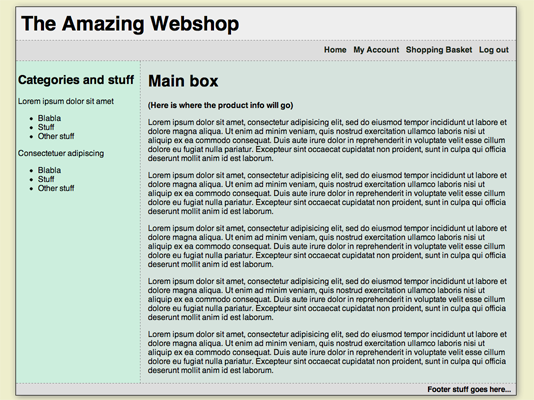
\includegraphics[width=10cm]{Screenshot_2012-11-16.png}
\caption{Screenshot of the webpage on November 16, 2012}
\label{fig:sshot}
\end{figure}

\subsubsection{References}
I used this guide:
\url{http://www.456bereastreet.com/lab/developing_with_web_standards/csslayout/2-col/}
when creating the website, it shows how to do a simple two-column webpage.

I used the CSS-information on \url{http://www.w3schools.com/} as a reference.

JQuery has excellent documentation available on \url{http://docs.jquery.com/}
and for positioning the shopping-basket information I used this addon: 
\url{http://docs.jquery.com/UI/API/1.8/Position}

\subsubsection{Converting the page to Django-templates}
The static skeleton-page has been converted into Django-templates.

Django rendering of pages consists of a few steps. First a url is defined in the
file \emph{urls.py}. This definition consists of a regexp that the url is matched
against and which method that should be invoked to handle the request.
\lstset{numbers=none}
\begin{lstlisting}
url(r'^ajax/addrating/(?P<productID>\d+)/(?P<grade>\d+)$',
	'shopping.views.asset_addgrade')}
\end{lstlisting}
\lstset{numbers=left}
In our project this means that the function \emph{asset\_addgrade()} in the module \emph{shopping} and the file \emph{views.py} is called when this url
is matched.

The regexp-groups in the url definition extract information from the url
and passes this information to the handler function. In our example the url
\emph{/ajax/addrating/1/4} would result in the function call:
\lstinline{asset_addgrade(request, productID=1, grade=4)}.
This function is expected to return an HTML response which it does
by gathering information from the request and from the database and what
other sources there might be and places this information in a context. 
It then renders a Django-template using this context and the output from the
render function is sent back to the client.

Django templating works by defining a template in a language that extends
HTML. The extension consists of certain tags that the template engine can
use to replace values or blocks of code. The template language supports
inheritance, so the user can define a base-file that contains all style-sheet and
javascript includes, the header, the footer, navigation etc and then use smaller
templates that extend this base-template to deal with the actual sub-pages of
the site.

An example of one of the sub-pages from the project looks like this:
\lstset{language=HTML}
\begin{lstlisting}



$(".buyproduct").click( function() {
$.get("/ajax/addproduct/" + this.id, function(data) {}); 
    $("#prodrow" + this.id).effect("transfer", {to: $(".arrowicon")}, 750);
});

 

<div class="catname">{{ category.name|capfirst }}</div>
<div class="catdesc">{{ category.description }}</div>
<div id="clear"></div>

<table id="product_list">

<tr id="prodrow{{product.pk}}" 
    class="">
        <td style="text-align: center;">
		<img src="{{product.image}}blank.png"/>
	</td>
        <td>
		<a href="/product/{{ product.pk }}">{{ product.name|capfirst }}</a>
	</td>
        <td> {{ product.description }} </td>
        <td> {{ product.stock }} in stock</td>
        <td> {{ product.price }} kr</td>
        <td style="text-align: right;">
		<button class="buyproduct" id="{{product.pk}}">Buy
		</button>
	</td>
</tr>

</table>

\end{lstlisting}
\lstset{language=Python}
This template extends \emph{base.html} so all the information surrounding
this content is already taken care of. \emph{base.html} defines a number of
``blocks'' where page-specific content can go. One of the blocks is
``js\_docready'' which is located in the javascript-part of \emph{base.html}.
The other block used in this template is the ``main''-block which is where, 
in \emph{base.html}, the main content area is defined.

The context provided to the template by the view-function can be used by the
template tags. For instance \emph{ \{\{ category.name|capfirst \}\} } will
get the attribute \emph{name} from the \emph{category}-object in the context
and then call the method \emph{capfirst}\footnote{This method makes the
first letter in a string a capital letter} with this information as the
argument. The output in the template will be the result of 
\emph{capfirst(category.name)}.

Similarly the template language supports loops and control sequences, as seen
in \emph{ \{\% for X in Y \%\} }, \emph{ \{\% endfor \%\} } and
\emph{ \{\% if condition \%\} }, \emph{ \{\% else \%\} }, \emph{ \{\% endif \%\} }, 

\subsection{Content management system}
The basic point of a CMS is to separate the administration of the website and
the editing of webpage code from the content. This allows users to edit the
webpage while focusing on the content and not the other details surrounding
a large site, especially the details of editing html and styling the content.


\section{Establish a relational database for e-commerce}
\subsection{Schema}

My schema consists of these entities:
\begin{itemize}
\setlength\itemsep{-7pt}
\item Customer
\item Category
\item Asset
\item Basket
\item BasketItem
\item Grade
\item GradeHistory
\item Comment
\end{itemize}
There is one additional entity which has a relationship to my model but isn't
defined by me. This is the \emph{User} entity that belongs to Django that I
extend using the Customer entity.

The relationships between these entities are as follows:
\begin{itemize}
\setlength\itemsep{-7pt}
\item \emph{Customer} extends \emph{User}
\item \emph{Asset} belongs to a \emph{Category}
\item \emph{BasketItem} belongs to a \emph{Basket}
\item \emph{BasketItem} contains an \emph{Asset}
\item \emph{Basket} belongs to a \emph{Customer}
\item \emph{Grade} belongs to an \emph{Asset}
\item \emph{GradeHistory} belongs to a \emph{Customer}
\item \emph{Comment} belongs to a \emph{Customer}
\item \emph{Comment} belongs to an \emph{Asset}
\end{itemize}

\subsubsection{Entity-Relationship Diagram}
The entity-relationship diagram created from this information and with the
attributes of the entities added can be seen in figure \ref{fig:erdiag}. 
The meaning of the different symbols is explained in this figure:
\begin{figure}[H]
\centering
\tikzstyle{every entity} = [top color=white, bottom color=blue!30, 
                            draw=blue!50!black!100, drop shadow]
\tikzstyle{every attribute} = [top color=white, bottom color=yellow!20, 
                               draw=yellow, node distance=1cm, drop shadow]
\tikzstyle{every relationship} = [top color=white, bottom color=green!20, 
                                  draw=green!50!black!100, drop shadow]
\begin{tikzpicture}[node distance=0.5cm, every edge/.style={link}]
% Legend
\node[entity] (leg_ent) [scale=0.65] {Entity};
\node[relationship] (leg_rel) [scale=0.65, right=of leg_ent] {\footnotesize{Relationship}};
\node[attribute] (leg_att) [scale=0.65, right=0.5cm of leg_rel] {Attribute};
%\node[draw,dashed,fit=(leg_ent) (leg_rel) (leg_att)] (leg_box) {};
\end{tikzpicture}
\caption{Legend for the ER-diagram (figure \ref{fig:erdiag})}
\end{figure}

\begin{figure}[H]
\centering
\tikzstyle{every entity} = [top color=white, bottom color=blue!30, 
                            draw=blue!50!black!100, drop shadow]
\tikzstyle{every attribute} = [top color=white, bottom color=yellow!20, 
                               draw=yellow, node distance=1cm, drop shadow]
\tikzstyle{every relationship} = [top color=white, bottom color=green!20, 
                                  draw=green!50!black!100, drop shadow]
\begin{tikzpicture}[node distance=1.5cm, every edge/.style={link}]
\node[entity] (cust) {Customer};
\node[relationship] (custusr) [above=of cust] {\footnotesize{\,\,\,Extends\,\,\,\,}} edge (cust);
\node[entity] (user) [bottom color=black!20, draw=black!40!black!60, dotted] [above=of custusr] {User} edge (custusr);

\node[entity] (asset) [right=5 cm of cust] {Asset};
\node[relationship] (asscat) [above=of asset] {\footnotesize{Belongs to}} edge (asset);
\node[entity] (category) [above=of asscat] {Category} edge (asscat);

\node[relationship] (bascus) [below right=1cm and 0.2cm of cust] {\small{Belongs to}} edge (cust);
\node[relationship] (basass) [below right=1.5cm and 1cm of asset] {\footnotesize{\,\,\,Contains\,\,\,}} edge (asset);

\node[entity] (basket) [below left=5cm and 3cm of basass] {Basket} edge (bascus);
\node[entity] (basketitem) [below left=0cm and 1.5cm of basass] {BasketItem}
edge (basass);

\node[relationship] (basitbas) [below right=1cm and 0.5cm of basketitem] {\small{Belongs to}}
edge (basketitem) edge (basket);

\node[entity] (gradehistory) [below left=5cm and -0.5cm of cust] {GradeHistory};
\node[entity] (grade) [above left=1.5cm and 1cm of asset] {Grade};

\node[relationship] (gradeass) [below right=1cm and -2cm of grade] {\small{Belongs to}}
edge (grade) edge (asset);
\node[relationship] (gradecust) [below left=of cust] {\footnotesize{Belongs to}}
edge(cust) edge(gradehistory);

\node[entity] (comment)  [below right=0cm and 1cm of gradehistory] {Comment};
\node[relationship] (custcomment) [below left=0.1cm and 1cm of bascus] {\footnotesize{Belongs to}} 
edge (cust) edge (comment);
\node[relationship] (asscomment) [above right=3cm and 1cm of comment] {\footnotesize{Belongs to}}
edge (comment) edge (asset);

% Customer attributes
\node[attribute] (address) [above left=1.25cm and 0.5cm of cust] {Address} edge (cust);
\node[attribute] (phone) [above left=0.25cm and 1.5cm of cust] {Phone} edge (cust);

% Asset attributes
\node[attribute] (name) [above right=1.25cm and 0.5cm of asset] {Name} edge (asset);
\node[attribute] (desc) [above right=0.25cm and 1.5cm of asset] {Description} edge (asset);
\node[attribute] (stock) [above right=-1cm and 1.5cm of asset] {Stock} edge (asset);

% Basket attributes
\node[attribute] (active) [below right=0.5cm and -1cm of basket] {Active baset} edge (basket);
\node[attribute] (dateordered) [below right=-0.5cm and 1cm of basket] {Order placed} edge (basket);
\node[attribute] (datefilled) [below right=-1.5cm and 1.5cm of basket] {Order filled} edge (basket);

% BasketItem attributes
\node[attribute] (count) [below left=0.5cm and -1cm of basketitem] {Count}
edge (basketitem);

% Grade attributes
\node[attribute] (gradecount) [above left=0.5cm and -1cm of grade] {Count} edge (grade);
\node[attribute] (gradesum) [above left=1.5cm and -2.5cm of grade] {Sum} edge (grade);

% GradeHistory attributes
\node[attribute] (ghhistory) [below left=1cm and -2cm of gradehistory] {history} edge (gradehistory);

% Comment attributes
\node[attribute] (timestamp) [below left=0.5cm and -1cm of comment] {timestamp} edge (comment);
\node[attribute] (ccomment) [below right=1.5cm and -1cm of comment] {comment} edge (comment);

% Category attributes
\node[attribute] (cname) [above left=1cm and 0cm of category] {Name} edge (category);
\node[attribute] (cdesc) [above right=1cm and 0cm of category] {Description} edge (category);
\end{tikzpicture}
\caption{Entity-relationship diagram}
\label{fig:erdiag}
\end{figure}

\subsection{Use cases}
I have tried to think of a few different use cases that might be typical for the
people interacting with the webshop.

\subsubsection{Browse category}

\begin{table}[H]
\centering
\begin{tabular}{r | p{12cm}}
\textbf{Title} & Browse category \\
\textbf{Actor} & User \\
\textbf{Goal} & Retrieve a list of all the products associated with a certain category \\
\textbf{Story} & The user clicks on one of the categories available from the sidebar and a new page is opened with a list of products \\
\end{tabular}
\caption{Browse category use-case}
\end{table}

\subsubsection{Purchase item}
\begin{table}[H]
\centering
\begin{tabular}{r | p{12cm}}
\textbf{Title} & Purchase item \\
\textbf{Actor} & User \\
\textbf{Goal} & Add an item to the shopping basket \\
\textbf{Story} & The user clicks on the purchase link/icon assiciated with the selected product and the product is added to the shopping basket\\
\end{tabular}
\caption{Purchase item use-case}
\end{table}

\subsubsection{Place order}
\begin{table}[H]
\centering
\begin{tabular}{r | p{12cm}}
\textbf{Title} & Place order \\
\textbf{Actor} & User \\
\textbf{Goal} & Place an order containing all of the items in the shopping basket \\
\textbf{Story} & The user is satisfied with the products in the shopping basket and opens the basket page by clicking on the link in the navigation panel.
A page showing order-confirmation with address and payment details is opened \\
\end{tabular}
\caption{Place order use-case}
\end{table}

\subsubsection{Fill order}
\begin{table}[H]
\centering
\begin{tabular}{r | p{12cm}}
\textbf{Title} & Fill order \\
\textbf{Actor} & Warehouse worker \\
\textbf{Goal} & Fill an order that is waiting for processing \\
\textbf{Story} & The warehouse worker opens a webpage that contains a list of
unprocessed orders, selects the one that has been waiting for the longest time and is shown a page where all the items, item-counts and customer shipping
details are shown. 
After retrieving all the ordered items and posting the box  the warehouse worker marks the order as placed\\
\end{tabular}
\caption{Fill order use-case}
\end{table}

\subsubsection{Change address}
\begin{table}[H]
\centering
\begin{tabular}{r | p{12cm}}
\textbf{Title} & Change address \\
\textbf{Actor} & User \\
\textbf{Goal} & Edit the address information stored in the database \\
\textbf{Story} & The user has moved to a new address and wishes to update
the information stored in the webshop. The user clicking on \emph{My Account}
in the navigation panel, edits the text-field with the address information and
clicks save \\
\end{tabular}
\caption{Fill order use-case}
\end{table}

\subsubsection{Add product}
\begin{table}[H]
\centering
\begin{tabular}{r | p{12cm}}
\textbf{Title} & Add product \\
\textbf{Actor} & Manager \\
\textbf{Goal} & Add a new product to the webshop \\
\textbf{Story} & A contract with a new supplier has been signed and new products need to be added to he shop. The manager goes to the administrative page and selects add product. A webform is presented where the manager enters the product information and uploads a picture \\
\end{tabular}
\caption{Add product use-case}
\end{table}

\subsubsection{Use-case diagram}
\begin{figure}[H]
\centering
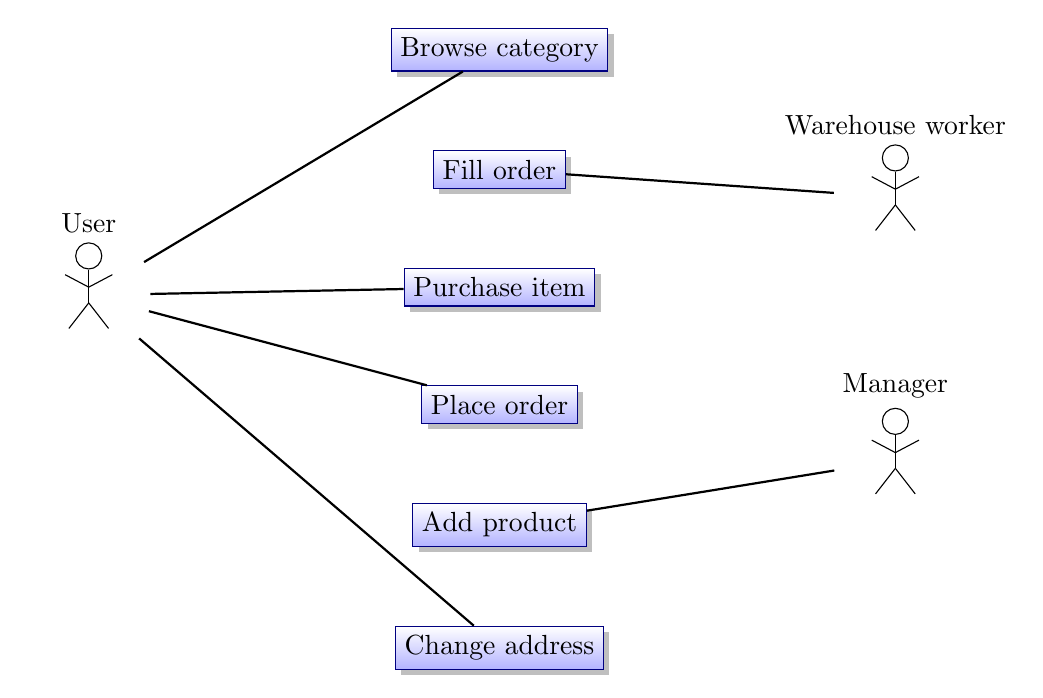
\begin{tikzpicture}[node distance=1cm]
% User
\node [draw, circle] (head1) {};
\node [below=0.3cm of head1] (midriff1) {};
\node [below=0.1cm of head1] (chestnode1) {};
\coordinate (mid1) at (midriff1);
\coordinate (chest1) at (chestnode1);
\node [below right=0.2cm and 0.1cm of midriff1] (rightleg1) {} edge (mid1);
\node [below left=0.2cm and 0.1cm of midriff1] (leftleg1) {} edge (mid1);
\draw  (mid1) -- (head1);
\node [above left=0.1cm and 0.3cm of chest1] (leftarm1) {} edge (chest1);
\node [above right=0.1cm and 0.3cm of chest1] (rightarm1) {} edge (chest1);
\node [above=0cm of head1] (label1) {User};
\node [ellipse, inner sep=0cm, fit=(head1) (midriff1) (chestnode1) (rightleg1) (leftleg1) (leftarm1) (rightarm1)] (personbox1) {};

% Use cases
%\node [draw] [right=4cm of chest1] [top color=white, bottom color=blue!30, draw=blue!50!black!100, drop shadow] 
%	(place) {Place order};
\node [draw] [right=4cm of chest1] [top color=white, bottom color=blue!30,  draw=blue!50!black!100, drop shadow] 
	(purchase) {Purchase item};
\node [draw] [above=of purchase] [top color=white, bottom color=blue!30,  draw=blue!50!black!100, drop shadow] 
	(fill) {Fill order};
\node [draw] [above=of fill] [top color=white, bottom color=blue!30,  draw=blue!50!black!100, drop shadow] 
	(browse) {Browse category};
%\node [draw] [below=of place] [top color=white, bottom color=blue!30,  draw=blue!50!black!100, drop shadow] 
%	(purchase) {Purchase item};
\node [draw] [below=of purchase] [top color=white, bottom color=blue!30, draw=blue!50!black!100, drop shadow] 
	(place) {Place order};
\node [draw] [below=of place] [top color=white, bottom color=blue!30,  draw=blue!50!black!100, drop shadow] 
	(addproduct) {Add product};
\node [draw] [below=of addproduct] [top color=white, bottom color=blue!30,  draw=blue!50!black!100, drop shadow] 
	(change) {Change address};

% User connections
\draw [thick] (personbox1) -- (browse);
\draw [thick] (personbox1) -- (purchase);
\draw [thick] (personbox1) -- (place);
\draw [thick] (personbox1) -- (change);

% Warehouse worker
\node [draw, circle] [above right=1cm and 10cm of head1]  (head2) {};
\node [below=0.3cm of head2] (midriff2) {};
\node [below=0.1cm of head2] (chestnode2) {};
\coordinate (mid2) at (midriff2);
\coordinate (chest2) at (chestnode2);
\node [below right=0.2cm and 0.1cm of midriff2] (rightleg2) {} edge (mid2);
\node [below left=0.2cm and 0.1cm of midriff2] (leftleg2) {} edge (mid2);
\draw  (mid2) -- (head2);
\node [above left=0.1cm and 0.3cm of chest2] (leftarm2) {} edge (chest2);
\node [above right=0.1cm and 0.3cm of chest2] (rightarm2) {} edge (chest2);
\node [above=0cm of head2] (label2) {Warehouse worker};
\node [ellipse, inner sep=0cm, fit=(head2) (midriff2) (chestnode2) (rightleg2) (leftleg2) (leftarm2) (rightarm2)] (personbox2) {};

% Warehouse worker connections
\draw [thick] (personbox2) -- (fill);

% Manager
\node [draw, circle] [below=3cm of head2]  (head3) {};
\node [below=0.3cm of head3] (midriff3) {};
\node [below=0.1cm of head3] (chestnode3) {};
\coordinate (mid3) at (midriff3);
\coordinate (chest3) at (chestnode3);
\node [below right=0.2cm and 0.1cm of midriff3] (rightleg3) {} edge (mid3);
\node [below left=0.2cm and 0.1cm of midriff3] (leftleg3) {} edge (mid3);
\draw  (mid3) -- (head3);
\node [above left=0.1cm and 0.3cm of chest3] (leftarm3) {} edge (chest3);
\node [above right=0.1cm and 0.3cm of chest3] (rightarm3) {} edge (chest3);
\node [above=0cm of head3] (label3) {Manager};
\node [ellipse, inner sep=0cm, fit=(head3) (midriff3) (chestnode3) (rightleg3) (leftleg3) (leftarm3) (rightarm3)] (personbox3) {};

% Manager connections
\draw [thick] (personbox3) -- (addproduct);
\end{tikzpicture}
\caption{Use-case diagram}
\label{fig:usecase}
\end{figure}

\subsection{Testing}
Some data is needed in the database to enable tests of the website.
Adding data to the database is currently done manually.

\subsubsection{Adding data to the database}
Django provides the ability to work with your application interactively through
the shell. This is very similar to working with an interactive python session but
also loads all the required Django-libraries.

To populate the database I have created this small script that is executed in the
django-shell environment:
\lstset{language=Python}
\begin{lstlisting}
from shopping.models import Customer, Category, Asset, Basket, Order

categories = [ 
        # (name, description)
        ('socks', 'Items to put on your feet'),
        ('shoes', 'Items to put on your socks'),
        ('fruit', "Eat this, it's good for you"),
        ('telephones', 'Put one end against your ear and shout in the other'),
]   

for n, d in categories:
    c = Category(name=n, description=d)
    c.save()

sockCat = Category.objects.get(name='socks')
shoeCat = Category.objects.get(name='shoes')
fruitCat = Category.objects.get(name='fruit')
telCat = Category.objects.get(name='telephones')
products = [ 
        # (name, description, category, stock)
        ('blue sock', 'An exquisite blue sock, fit for kings and queens alike', sockCat, 3), 
        ('green sock', 'A sock of the green persuasion', sockCat, 10),
        ('gray sock', 'This sock lacks color', sockCat, 7), 

        ('boot', 'A boot (or two boots to be specific)', shoeCat, 5), 
        ('loafer', 'A loafer, slip it on and forget all about it', shoeCat, 3), 
    
        ('banana', 'A yellow fruit, not very round at all', fruitCat, 24),
        ('pear', 'This fruit is a bit more round than the banana', fruitCat, 13),
        ('apple', "Currently this is the roundest fruit we've got!", fruitCat, 7), 

        ('fixed phone', "This is where it's at", telCat, 10),
        ('mobile phone', "Everywhere is where it's at", telCat, 10) 
]   

for n, d, c, s in products:
    a = Asset(name=n, description=d, category=c, stock=s)
    a.save()
\end{lstlisting}
This creates a number of categories and then a number of assets which
belong to the different categories.

\subsection{Tools and references}
The diagrams were created using the \LaTeX-package
``Ti\emph{k}Z'', which I've used before and is great in many ways for diagram
drawing and data plotting. The Ti\emph{k}Z-manual\footnote{\url{http://www.texample.net/media/pgf/builds/pgfmanualCVS2012-11-04.pdf}} 
contains in depth detail and there are plenty of different 
Ti\emph{k}Z-examples on the \TeX ample.net-page\footnote{
\url{http://www.texample.net/tikz/examples/}} (including an ER-diagram example).

\section{Shopping basket}
The way I have chosen to do the shopping basket is to have a basket that is
bound to the user and saved in the database so that it persists between
sessions.
This means that a user can log on, browse for a while, add some products to
the basket and then log out. The next time that user logs on the basket will
still be there.

When a user buys a product there are two steps involved. The first step is
placing the product in the basket and the second step is placing the actual
order. Since products are limited by the number stored in the warehouse,
it is important to choose whether to reserve the product when it is added
to the basket, or to check if there are sufficient numbers of the product in 
stock at the time of placing the order.

Since the basket is stored between sessions in this case, it was an easy choice.
Updating stock on the product when placing it in the basket could mean
reserving it indefinitely, which is not good at all.
The right thing to do in this case is to hold off on that check until the order
is placed. This could mean that the user can't order the items because they
are out of stock, but this is a natural scenario and easily remedied by going
back to the basket and updating the amount.

\subsection{Implementation}
The basket is implemented by adding two new tables in the database.
Firstly there is the \textsc{Basket} table, which is defined through this model:
\begin{lstlisting}
class Basket(models.Model):
	"""
	Shopping basket, 
	Belongs to a customer, contains a flag for whether it is an 
	active basket or an order, and timestamps.
	"""
	customer = models.ForeignKey(Customer)
	# Active = current basket, inactive = order
	active = models.BooleanField(default=True) 

	# These two fields are only interesting when the basket 
	# becomes an order:

	# Date the order was placed
	date_placed = models.DateTimeField(null=True, blank=True) 

	# Date the order was filled 
	date_filled = models.DateTimeField(null=True, blank=True) 
\end{lstlisting}
The basket has two functions. If the attribute $active$ is \emph{True} then 
the basketis the current shopping basket. 
If no current shopping basket exists then one will be created automatically
when the user performs any action on the webpage that requires a shopping basket.

If $active$ is \emph{False}, then the basket is an order. When the user selects 
``place order'' and the order has been validated the flag is switched from
\emph{True} to \emph{False} and $date\_placed$ is set to the current date and time.

When a warehouse worker needs to see which orders need attention, a query 
on \textsc{Basket}s for rows where $date\_filled$ is not set will give a list
of orders that are waiting for shipping. After the products have been packed
and shipped the warehouse worker updates the field and sets it to the current
date and time.

The second new model is \textsc{BasketItem}. 
\begin{lstlisting}
class BasketItem(models.Model):    
	"""    Maps assets to the basket
	"""
	basket = models.ForeignKey(Basket)
	asset = models.ForeignKey(Asset)
	count = models.IntegerField(default=0)
(self.asset)
\end{lstlisting}
This table is basically a mapping between \textsc{Basket} and \textsc{Asset}.
When a user adds an asset to the shopping basket, we first query the database
for a \textsc{BasketItem}-entry with the users current \textsc{Basket} and the 
current \textsc{Asset}. If such an entry exists then the $count$-field is
incremented by one and the entry saved back to the database.
It no such entry exists a new \textsc{BasketItem} is created with $count$
initialized to 0.


\section{Grading}

There are a few different ways to implement rating of products. I will examine
three methods and their merits/weaknesses.
\subsection{One row per grade}
The first method is to create a table with three columns (\emph{id} implied): 
\begin{description}
\setlength\itemsep{-7pt}
\item[asset] Foreign key into the \textsc{Asset} table
\item[customer] Foreign key into the \textsc{Customer} table
\item[grade] The rating itself (a number between 1 and 5)
\end{description}
Every time a grade is added a new row is appended to this table.

Calculating the grade of a product consists of fetching all the rows where 
$asset = productID$, adding together all the $grade$s and dividing by the
$count$ of the rows.

The advantage of this system is that every review is traceable, you always
know what rating a customer gave to a specific product. It is easy to prevent
a user from rating a product more than once and the user could even have the
ability to change the grade.

The disadvantage is that if there are $n$ customers and $m$ products, and all
customers grade every product there will be $n*m$ rows in this table.
Furthermore, every time a product-page is fetched and the review is calculated
we would have to fetch up to $n$ rows from the table to calculate the grade.

\subsection{Low impact implementation}
The second way is to simply keep a table with these attributes:
\begin{description}
\setlength\itemsep{-7pt}
\item[asset] Foreign key into the \textsc{Asset} table
\item[count] The number of votes
\item[sum] Total sum of all ratings
\end{description}
Every time a product is rated the row with the correct $asset$ will have its
$count$-field incremented by $1$ and the grade will be added to the $sum$. 

Calculating the grade consists of fetching the one row from the database
with the correct $asset$ and then evaluating $\frac{sum}{count}$.

This has the advantage of being fast and easy to implement. Fast because every
time a rating needs to be fetched only one row needs to be retrieved and only
one calculation performed.
The disadvantage is that a customer can keep rating the same product over and
over again and thus skewing the total grade of the product.

\subsection{The compromise}
The third option is a compromise between the two previous methods.
In the same way as the ``low impact method'' a grade-table is kept that
consists of $asset$, $count$ and $sum$.

However, to prevent users rating the same product over and over there is a
second table, \textsc{GradeHistory}, that has two fields.
\begin{description}
% TODO: table, \caption{ \textsc{Grade}-able in the final method}
\setlength\itemsep{-7pt}
\item[customer] Foreign key into the \textsc{Customer} table
\item[history] A comma-separated list of productID's that the user has rated
\end{description}
When a customer tries to rate a product, that customers' 
\textsc{GradeHistory}-row is fetched and a check is done to see if productID is
in the history-list. If it is, the rating is rejected. If it is not, the grade is
accepted and the productID is added to the history.

The same problem exists here, what if all $n$ customers rate all $m$ products?
Then the history field would become very big. It will still only be one row that
we need to fetch to perform the check.
Limiting the size of the history-field is easy, one can simple settle with keeping
a history of the last k grades, and if adding the grade to history causes it to be
of length k+1 then \emph{pop()}-ing the fist grade will keep it in check. 

This way a user can still vote more times for the same product, but
only after having first voted for $k$ number of other products not in the
 $history$-list. 

In reality, since $history$ is a list of productID's, and is stored as a 
\emph{varchar} in the database, setting $k$ can't be done exactly.
For instance, if productID is only a single digit (``$1,2,3,4$'') then storing 
$4$ values would take $4\cdot 2 - 1$ characters. But what if there are
thousands of products, with productID's such as $9387$. Then we can store
fewer values in the $history$-list.

I have chosen to live with this ``soft'' limit and set the maximum length of
the history to something relatively big, $1000$ characters in this case.

Fetching a grade consists of getting the  one correct row from the 
\textsc{Grade}-table and evaluating $\frac{sum}{count}$, one read and one
calculation.
Adding a grade fetches the row from \textsc{Grade} but also fetches the \textsc{GradeHistory}-row and checks if the user has already
voted for this product.

With this method the database won't grow out of control with a large number 
of users and products but there are still some limitations on what the users 
can do.

\subsubsection{The implementation}
The two models that have been added are \textsc{Grading} and 
\textsc{GradeHistory}. These look like this:
\begin{lstlisting}
class Grade(models.Model):
    """
    Product ratings
    """ 
    asset = models.ForeignKey(Asset)
    count = models.IntegerField(default=0)  # Total number of grades
    sum = models.IntegerField(default=0)    # Total sum of all grades
\end{lstlisting}
\begin{lstlisting}
class GradeHistory(models.Model):
    """
    A customers rating-history
    """ 
    customer = models.ForeignKey(Customer)
    history = models.CharField(max_length=1000, default="")
\end{lstlisting}

When a product page is loaded, the related \textsc{Grade}-row is queried.
If no rating has been given to the product yet a message about that will be
shown. If there are ratings, the average is calculated and a tuple consisting of
$(average rating, number of votes)$ is passed on to the template and shown.

When a user gives a rating to a product (by selecting a number between 1 and 5
in a dropdown box on the product page and then clicking the Rate-button) 
an ajax call is done. The method invoked this way will first get the users
\textsc{GradeHistory} row, or create it if it doesn't exist yet.
If the current productID is found in the $history$-attribute of the
\textsc{GradeHistory}-entry then the user is not allowed to rate the product,
and an error message will be shown. If the $history$-attribute does not contain
the product then the products \textsc{Grade}-row is loaded (or created if 
it doesn't exist) and the $count$ and $sum$ fields are updated.

\section{Comments}
Comments are implemented using a single level of commenting, at this time
there is no support for leaving a reply to a comment and having it show up
as a related comment (see section~\ref{sec:related_comments} for the 
reason why).

\subsection{Implementation}
The following model has been added:
\begin{lstlisting}
class Comment(models.Model):
    """ 
    Comment on a product
    """
    asset = models.ForeignKey(Asset)
    customer = models.ForeignKey(Customer)
    timestamp = models.DateTimeField(auto_now_add=True)
    comment = models.CharField(max_length=500)
\end{lstlisting}
Since there can be many comments on a product and we want to keep the time
from when the page is requested until it is loaded in the clients browser as
short as possible the comment-section of the product page is fetched by an
ajax call. This means that the product-page will load and then the comments
are loaded and placed in the comment-area.

When a comment is added an javascript function takes the content of the
comment-box and uses ajax to call a function that validates the comment.
If something is wrong with the comment, an error message is shown.
If everything was okay with the comment, it is added to the database and the
comment-section is reloaded using ajax.

\subsection{Related comments}
\label{sec:related_comments}
I started implementing related comments. 
The way I did this is by adding a field to the \textsc{Comment}-model called
$related\_to$. This field was a foreign key pointing back into \textsc{Comment}.
If a comment is a reply to another comment then this field would be set to the
$id$ of that comment and if the comment was a new comment and not related
to other comments any way then the field would not be set.

Building the tree of comments consisted of getting all the comments for the
current asset and then recursively building the comment-structure, like this
algorithm:
\begin{lstlisting}

all_comments = Comment.objects.filter(asset__pk = productID)

base_comments = all_comments.filter(related_to = None)

# Iterate over all base (level 0) comments
for base_comment in base_comments:
	# Fetch the comments that are directly children to this
    	children = build_children_tree(all_comments, base_comment)
    	comment_list.append( (base_comment, children) )

def build_children_tree(all_comments, base_comment):
	"""
	Recursively build the comment tree
	"""
	# Remove the current comment from the list 
	# to speed up things a bit later:
	all_comments.remove(base_comment) 

	list = []
	children = all_comments.filter(response_to = base_comment)
	if len(children) == 0:
		return None
	for child in children:
		grandchildren = build_children_tree(all_comments, child)
		list.append (child, grandchildren)
	return list
\end{lstlisting}
The comment structure is a list of tuples: $(comment, [children])$ or 
$(comment, None)$ if the comment has no children.
Replacing the comment-objects with example comments it would look 
something like this:
\begin{verbatim}
[
  ("Denna produkt är bra", None),
  ("Denna produkt är dålig", [ 
      ("Varför det?", [
          ("Därför att jag säger så", None)
          ]) 
  ]),
  ("Det här är en orelaterad kommentar", None)
]
\end{verbatim}

At this point I realized that Django-templates do not support recursion, 
so rendering of comments would have to be done by generating the 
HTML-code inline. Ofcourse you could still utilize the template-engine and
render each level of recursion separately with a call to $render()$, but I decided
to focus on other things instead for the time being. I might come back to this.




\end{document}
